%TEMPLATE
\begin{comment}	
	\begin{question}[name=Oppgave, topic=zenerdioder]
		
	\end{question}
	
	\vspace{0.5cm} % Add space after the solution
	
	\begin{solution}[name=Løsningsforslag oppgave]

	\end{solution}
\end{comment}


\begin{question}[name=Oppgave, topic=zenerdioder]
Hvilken side er katode, og hva heter den andre siden vist i Figur \ref{fig:zenBasic}.

	\begin{figure}[H]
	\centering
	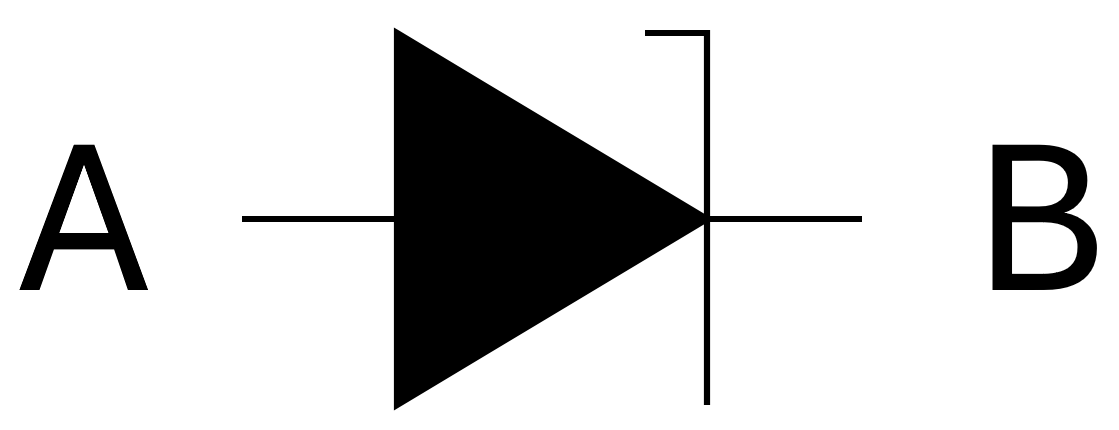
\includegraphics[width=0.3\textwidth]{diode/figurer/zenBasic.png}
	\caption{Symbol for Zenerdiode}
	\label{fig:zenBasic}
	\end{figure}

\end{question}

\vspace{0.5cm} % Add space after the solution

\begin{solution}[name=Løsningsforslag oppgave]
A er andode mens B er katode.

\end{solution}

\begin{question}[name=Oppgave, topic=zenerdioder]


\begin{enumerate}[label=\roman*)]
	\item Hva er den viktigste begrensingen i bruk av zenerdiode i en krets?
	\item Hvordan kan man beskytte en zenerdiode mot overbelastning?
\end{enumerate}

\end{question}

\vspace{0.5cm} % Add space after the solution

\begin{solution}[name=Løsningsforslag oppgave]
\begin{enumerate}[label=\roman*)]
	\item Zenerdiodens merke-effekt og merkestrøm. Om man går over disse grenseverdiene vil zenerdioden kunne bli skadet.
	\item Benytte en seriemotstand med korrekt resistans slik at strømmen blir begrenset for å beskytte zenerdioden.
\end{enumerate}

Zenerdiodens merke-effekt og merkestrøm. Om man går over disse grenseverdiene vil zenerdioden kunne bli skadet.
\end{solution}


\begin{question}[name=Oppgave, topic=zenerdioder]
En zenerdiode er merket 6V2/3W. Hva er den maksimale strømmen zenerdioden kan tåle?
\end{question}

\vspace{0.5cm} % Add space after the solution

\begin{solution}[name=Løsningsforslag oppgave]
\[P=U\cdot I\rightarrow I=\frac{P}{U}=\frac{3}{6,2}=484 [mA]\]
	
\end{solution}



\begin{question}[name=Oppgave, topic=zenerdioder]
En likespenning som varierer mellom $18 [V]$ og $24 [V]$ skal benyttes for å generere en stabil likespenning på $7,5 [V]$. Kretsen skal benytte en zenerdiode som tåler en effekt på maksimalt $4 [W]$.

\begin{enumerate}[label=\roman*)]
	\item Tegn opp kretsen
	\item Beregn den minste verdien seriemotstanden kan ha
	\item Beregn størrelsen på strømmen det maksimalt kan trekkes fra den stabiliserte spenningen på utgangen, før utgangsspenningen avviker fra $7,5 [A]$
\end{enumerate}
\end{question}

\vspace{0.5cm} % Add space after the solution

\begin{solution}[name=Løsningsforslag oppgave]
\begin{enumerate}[label=\roman*)]
	\item Figur \ref{fig:zenKrets1} viser ett eksempel på hvordan kretsen kan tegnes.
		\begin{figure}[H]
			\centering
			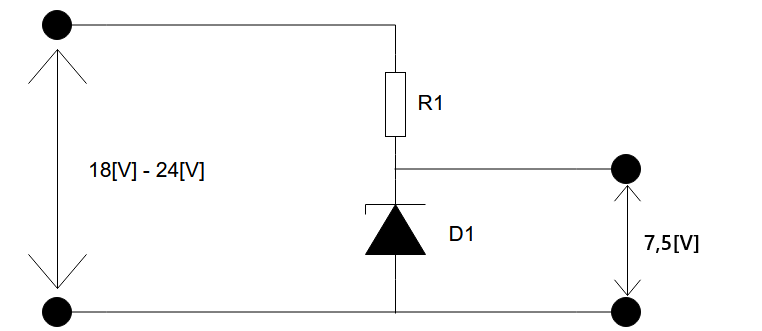
\includegraphics[width=0.7\textwidth]{diode/figurer/zenKrets1.png}
			\caption{Krets for spenningsstabilisering}
			\label{fig:zenKrets1}
		\end{figure}
	\item Beregner den minste verdien motstanden kan ha slik at strømmen i kretsen ikke blir større enn hva zenerdioden tåler. Starter med å finne den maksimale strømmen dioden tåler.
	
	\[I_{D_{maks}}=\frac{P}{U_{maks}}=\frac{4}{7,5}=\frac{8}{15}\approx 0,53 [A]\]
	
	Finner minste verdi for serieresistansen som vil resultere i å begrense strømmen i kretsen akuratt slik at zenerdioden ikke arbeider utenfor arbeidsområdet sitt ved maksimal spenning og strøm.
	
	\[R_{min}= \frac{U_{maks}}{I_{maks}}= \frac{24-7,5}{0,53} \approx 31 [\Omega]\]
	
	\item Når strømmen overgår verdien som resulterer i at man overgår effektbegrensingen til zenerdioden, så vil man ikke lenger garantere at zenerdioden klarer å holde spenningen konstant. Den maksimale strømmen har vi alt beregnet.
	
	\[I_{D_{maks}} \approx 533 [mA]\]
\end{enumerate}
\end{solution}


\begin{question}[name=Oppgave, topic=zenerdioder]
Kretsen vist i Figur \ref{fig:zenKrets2} viser en zenerdiodekrets konstruert for å holde spenningen ut stabil på $10[V]$. I følge databladet til zenerdioden har den følgende data:

\[I_{Zen_{min}}= 4 [mA]\]
\[I_{Zen_{maks}}= 40 [mA]\]

\begin{enumerate}[label=\roman*)]
	\item Beregn den maksimale spenningen for $U_{inn}$
	\item Beregn den minste spenningen for $U_{inn}$
\end{enumerate}
	
	
\begin{figure}[H]
	\centering
	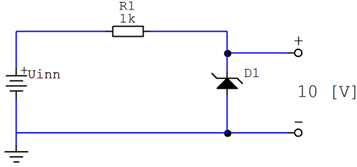
\includegraphics[width=0.5\textwidth]{diode/figurer/zenKrets2.png}
	\caption{Krets for spenningsstabilisering}
	\label{fig:zenKrets2}
\end{figure}

\end{question}

\vspace{0.5cm} % Add space after the solution

\begin{solution}[name=Løsningsforslag oppgave]
\begin{enumerate}[label=\roman*)]
	\item Beregner først det største spenningsfallet vi kan ha over resistansen $R_1$.
\[U_{R_{1}}=I_{Zen_{maks}} \cdot R_1=40 \cdot 10^{-3} \cdot 1 \cdot 10^3= 40[V]\]

	Beregner så den maksimale spenningen kretsen kan ha på inngangen.
\[U_{inn_{maks}}=U_{R_{1}}+U_{D_{1}}=40+10=50 [V]\]

	\item Beregn den minste spenningen for $U_{inn}$
\[U_{R_{1}}=I_{Zen_{min}} \cdot R_1=4 \cdot 10^{-3} \cdot 1 \cdot 10^3= 4[V]\]

Beregner så den maksimale spenningen kretsen kan ha på inngangen.
\[U_{inn_{min}}=U_{R_{1}}+U_{D_{1}}=4+10=14 [V]\]	

\end{enumerate}	
\end{solution}


\begin{question}[name=Oppgave, topic=zenerdioder]
Zenerdioden vist i Figur \ref{fig:zenKrets3} tåler en effekt på $5 [W]$. Beregn den minste verdien serieresistansen $R_1$ kan ha for at ikke zenerdioden skal bli utsatt for høyere effekt enn merkeverdien.
\begin{figure}[H]
	\centering
	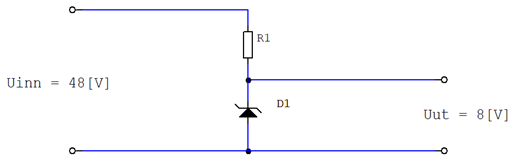
\includegraphics[width=0.7\textwidth]{diode/figurer/zenKrets3.png}
	\caption{Krets for spenningsstabilisering}
	\label{fig:zenKrets3}
\end{figure}	
\end{question}

\vspace{0.5cm} % Add space after the solution

\begin{solution}[name=Løsningsforslag oppgave]
Finner den totalte strømmen som går gjennom kretsen ved merkeeffekt på dioden.

\[I_{D_{maks}} = \frac{P_D}{U_D} = \frac{5}{8} = 0.625 = 625 [mA]\]


Finner så verdien motstanden må ha for å begrense strømmen slik at zenerdioden ikke blir utsatt for en effekt over merkeeffekt.


\[R_1 = \frac{U_{R_1}}{I_{R_1}}= \frac{48-8}{0,625}= 64 [\Omega]\]
\end{solution}



\begin{question}[name=Oppgave, topic=zenerdioder]
Zenerdioden i kretsen som vist i Figur \ref{fig:zenKrets4} har en zenerspenning på $5,1 [V]$. Zenerdioden er koblet i serie med en motstand på $33 [\Omega]$. Spenningen ut fra kilden $U_{inn}$ varierer mellom $9[V]$ og $10 [V]$.

Finn den minste effekten zenerdioden må tåle.
\begin{figure}[H]
	\centering
	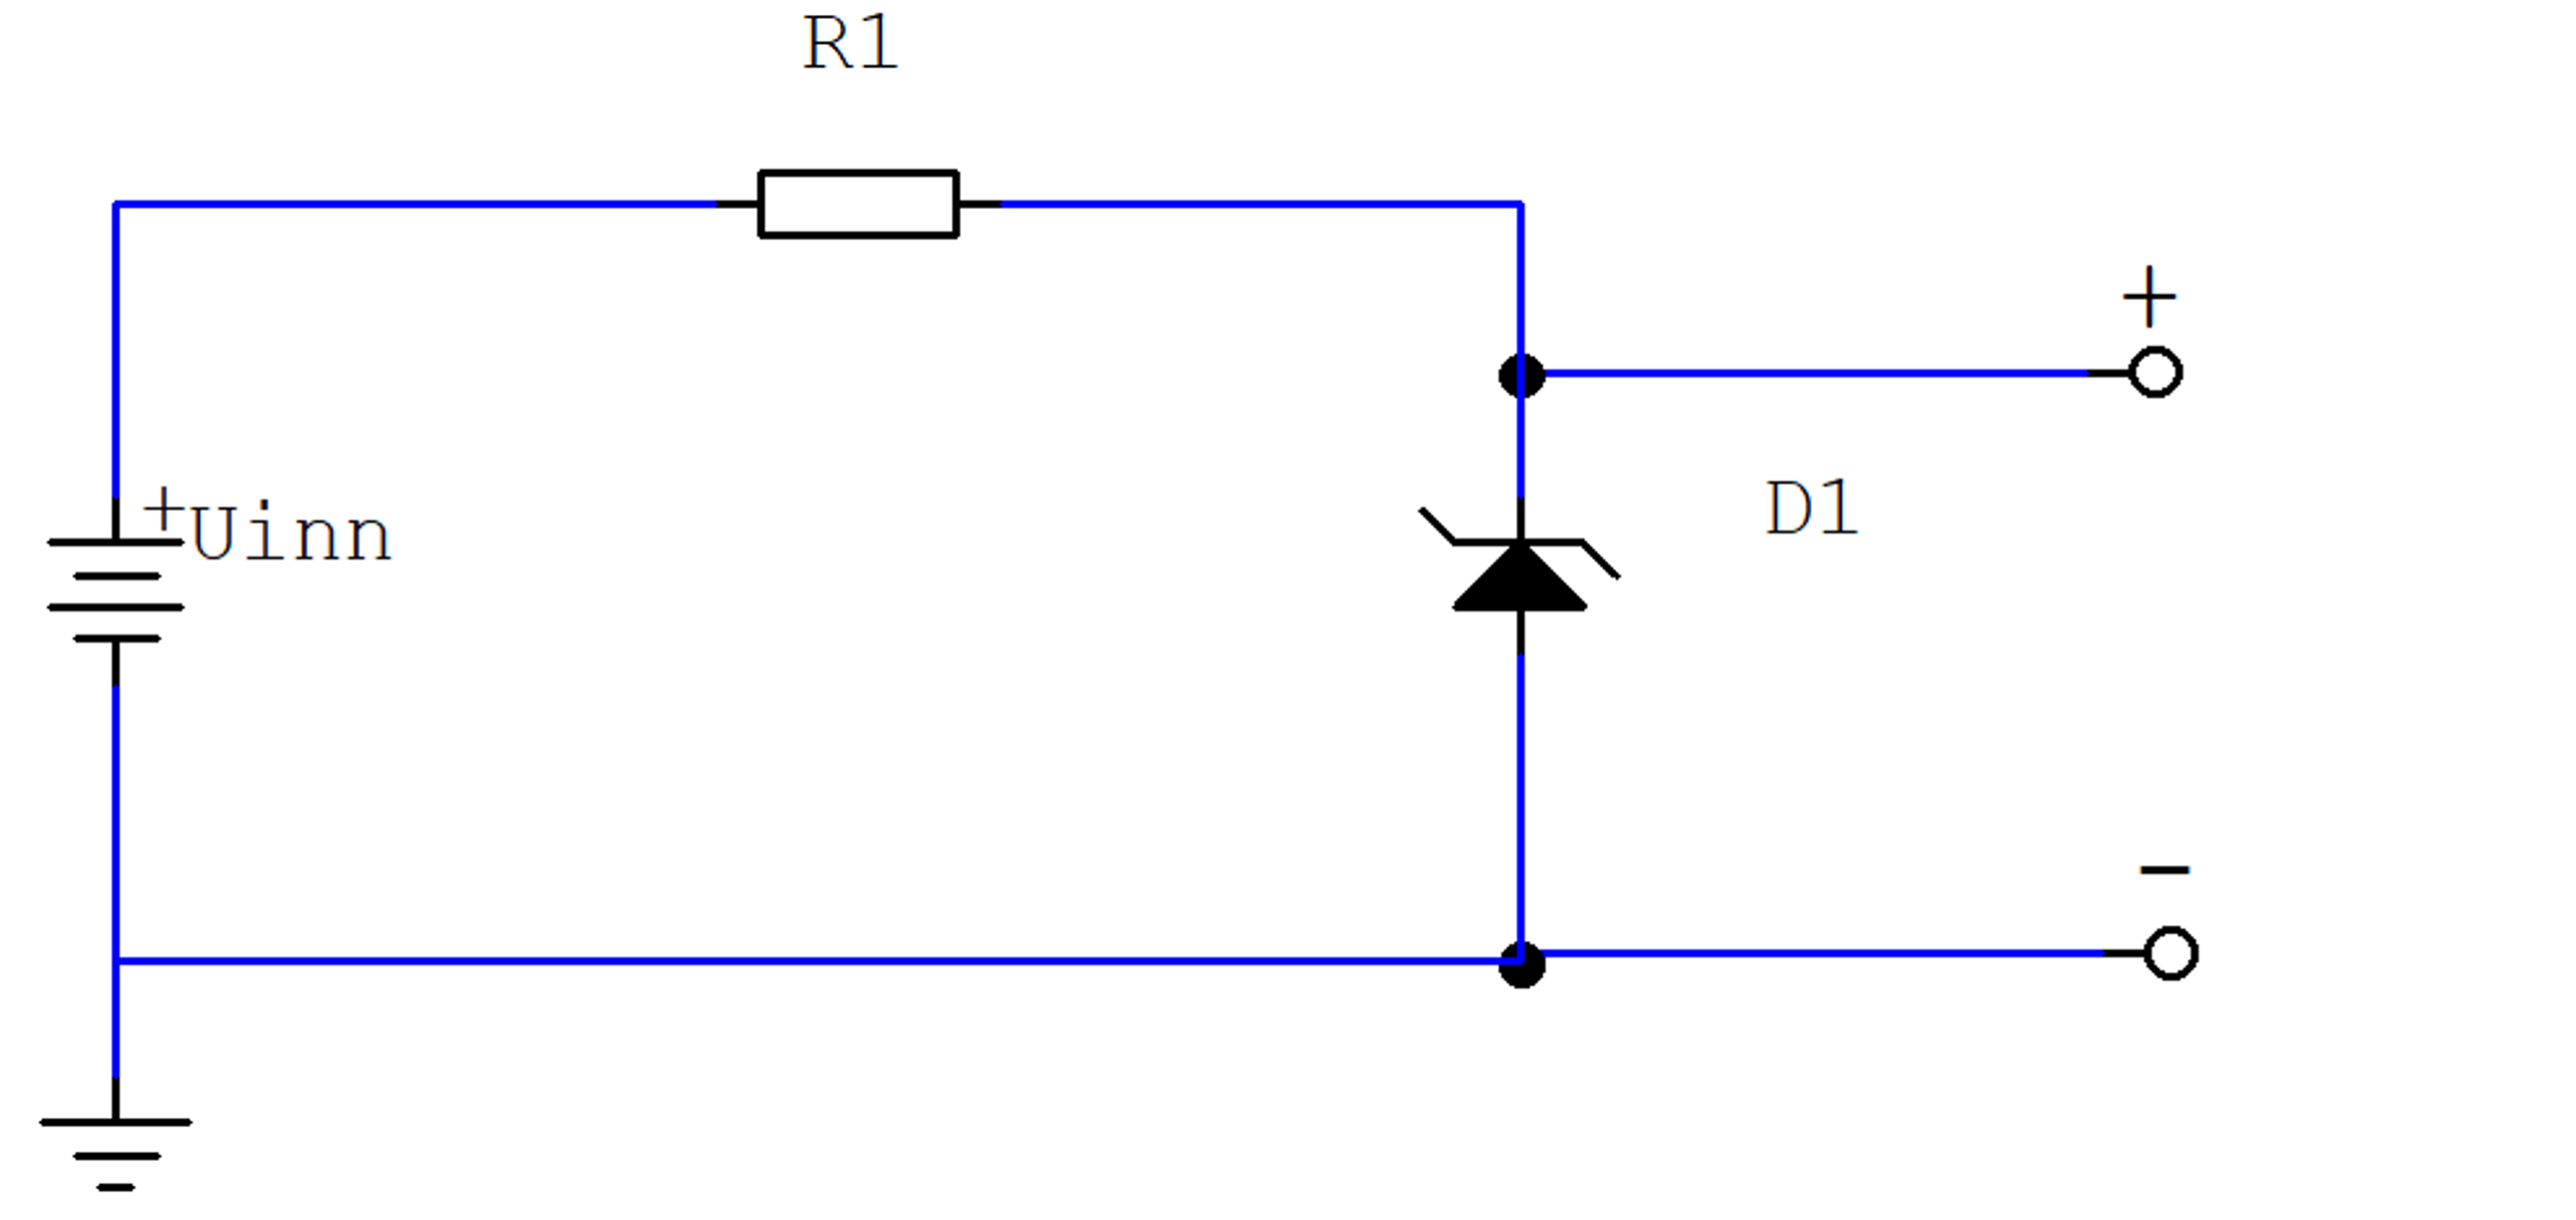
\includegraphics[width=0.7\textwidth]{diode/figurer/zenKrets4.png}
	\caption{Krets for spenningsstabilisering}
	\label{fig:zenKrets4}
\end{figure}	

\end{question}

\vspace{0.5cm} % Add space after the solution

\begin{solution}[name=Løsningsforslag oppgave]
Verstetilfelle og dimmensjonerende verdi blir med maksimal spenning ut fra spenningskilden ved $10 [V]$.

Beregner spenningsfallet over motstanden.
\[U_R=U_{inn}-U_{zen}=10-5,1=4,9[V]\]
	
Beregner strømmen som går i kretsen ved maksimal spenning ut fra spenningskilden.
\[I_{maks}=\frac{U_R}{R}=\frac{4,9}{33} \approx0,148 = 148 [mA]\]

Beregner effekten som blir omsatt under disse forholdene.
\[P_{zen}=U_{zen}\cdot I_{zen}= 4,9\cdot 150\cdot 10^{-3}=735[mW]\]
	
\end{solution}





